%%%%%%%%%%%%%%%%%%%%%%%%%%%%%%%%%%%%% 
%% LE2I beamer template
%% Guillaume Lemaitre, October 2014
%%%%%%%%%%%%%%%%%%%%%%%%%%%%%%%%%%%%% 

\documentclass{beamer}

\usepackage[utf8]{inputenc}
\usepackage[T1]{fontenc} 
\usetheme{le2i} 

%% The amssymb package provides various useful mathematical symbols
\usepackage{amssymb}
%% The amsthm package provides extended theorem environments
\usepackage{amsthm}
%% amsmath for math environment
\usepackage{amsmath}

\DeclareMathOperator*{\argmin}{arg\,min}
\DeclareMathOperator*{\argmax}{arg\,max}
\DeclareMathOperator*{\sign}{sign}

%% figure package
\usepackage{epsf,graphicx}
\usepackage{epstopdf}
\usepackage{subfigure}
\usepackage{transparent}

%% In order to draw some graphs
\usepackage{tikz,xifthen}
\usepackage{tikz-qtree}
\usepackage{adjustbox}
\usetikzlibrary{decorations.pathmorphing}
\usetikzlibrary{fit}
\usetikzlibrary{backgrounds}
\usetikzlibrary{shapes,arrows,shadows}
\usetikzlibrary{calc,decorations.pathreplacing,decorations.markings,positioning}
\usetikzlibrary{snakes,decorations.text,shapes,patterns}
% \usepackage{scalefnt,lmodern,booktabs}

%% Package for cross and tick symbols
\usepackage{pifont}
\newcommand{\tick}{\color{green!60!black!80}\ding{51}}
\newcommand{\cross}{\color{red!60!black!80}\ding{55}}

\title{Digital Electonic}
\author{Cédric Lemaître \\ \texttt{c.lemaitre58@gmail.com}}
\date{BScv 2016 - 2017 \\ 2\textsuperscript{nd} semester}

\institute{Universit\'e de Bourgogne} 

%% Uncomment if you want to avoid thousand of bullet inside the menu
% \usepackage{etoolbox}
% \makeatletter
% \patchcmd{\slideentry}{\advance\beamer@xpos by1\relax}{}{}{}
% \def\beamer@subsectionentry#1#2#3#4#5{\advance\beamer@xpos by1\relax}%
% \makeatother

\begin{document}

% Show the title page
\begin{frame}
  \titlepage
\end{frame}

% Show the table of contents
\begin{frame}
  \tableofcontents[sectionstyle=show,subsectionstyle=show,subsubsectionstyle=hide]
\end{frame}

\section{Digital Electonic Basics}

\subsection{Considering a real problem}

\begin{frame}
  \frametitle{Digital Electronics Basics}
  \framesubtitle{Considering a real problem}
  \begin{block}{Problem}
	  A tank is filled by 2 pipes : $V_1$ and $V_2$.
	  We consider 3 levels
    \begin{itemize}
	\item Warning (W)
	\item Bottom (B)
	\item top (T)
    \end{itemize}
    When level is behind W, $V_1$ et $V_2$ are opened.\\
    When level is between W and B, only $V_1$ is opened.\\
    When level is between B and T, only $V_2$ is opened.\\
    When level is upper T, we close the pipe.
  \end{block}

  %  \begin{figure}
  %    \centering
  %    
\includegraphics[width=.2\textwidth]{./images/logos/le2i-logo.pdf}
  %    \caption{Include an image}
  %  \end{figure}
\end{frame}

\begin{frame}
  \frametitle{Digital Electronics Basics}
  \framesubtitle{Considering a real problem}
  \begin{block}{How to do?}
	  \begin{itemize}
		  \item Make a drawing
	  \end{itemize}
\end{block}
\end{frame}


\begin{frame}
  \frametitle{Digital Electronics Basics}
  \framesubtitle{Considering a real problem}
  \begin{block}{How to do?}
	  \begin{itemize}
		  \item Make a drawing
		\item Make the truth table
	  \end{itemize}
\end{block}
\end{frame}

\begin{frame}
  \frametitle{Digital Electronics Basics}
  \framesubtitle{Considering a real problem}
  \begin{block}{How to do?}
	  \begin{itemize}
		  \item Make a drawing
		\item Make the truth table
		\item Reduice complexity by using Karnaugh table and rules
	  \end{itemize}
\end{block}
\end{frame}


\begin{frame}
  \frametitle{Digital Electronics Basics}
  \framesubtitle{Considering a real problem}
  \begin{block}{Implementation using Electronic component}
    \begin{itemize}
	\item Which Family? CMOS or TTL technology?
    \end{itemize}
  \end{block}

    \begin{figure}
      \centering
      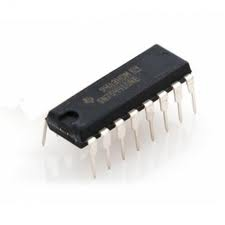
\includegraphics[width=.2\textwidth]{./images/ttl_7406.png}
      \caption{TTL 7406}
    \end{figure}
\end{frame}


\begin{frame}
  \frametitle{Digital Electronics Basics}
  \framesubtitle{Techno - information}


 \begin{columns}[t]
	 \begin{column}{5cm}
		\begin{block}{TTL}
			\begin{itemize}
				\item Input voltage 5V +-5\%
				\item 0 : 0.4V--0.8V
				\item 1 : 2.4V--2.8V
				\item TP : 10ns for "N" series and 1.5ns for "AS"
			\end{itemize}
		\end{block} 
	\end{column}
					   
	\begin{column}{5cm}
		\begin{block}{CMOS}
			\begin{itemize}
				\item Input voltage 3 to 18v
				\item 0 : 0.05Vcc--0.45Vcc 
				\item 1 : 0.55Vcc--0.95Vcc
				\item TP : depending of Vcc
			\end{itemize}
		\end{block}   
	\end{column}
\end{columns}  
\end{frame}

\begin{frame}
  \frametitle{Digital Electronics Basics}
  \framesubtitle{Techno - information}
    \begin{figure}
      \centering
      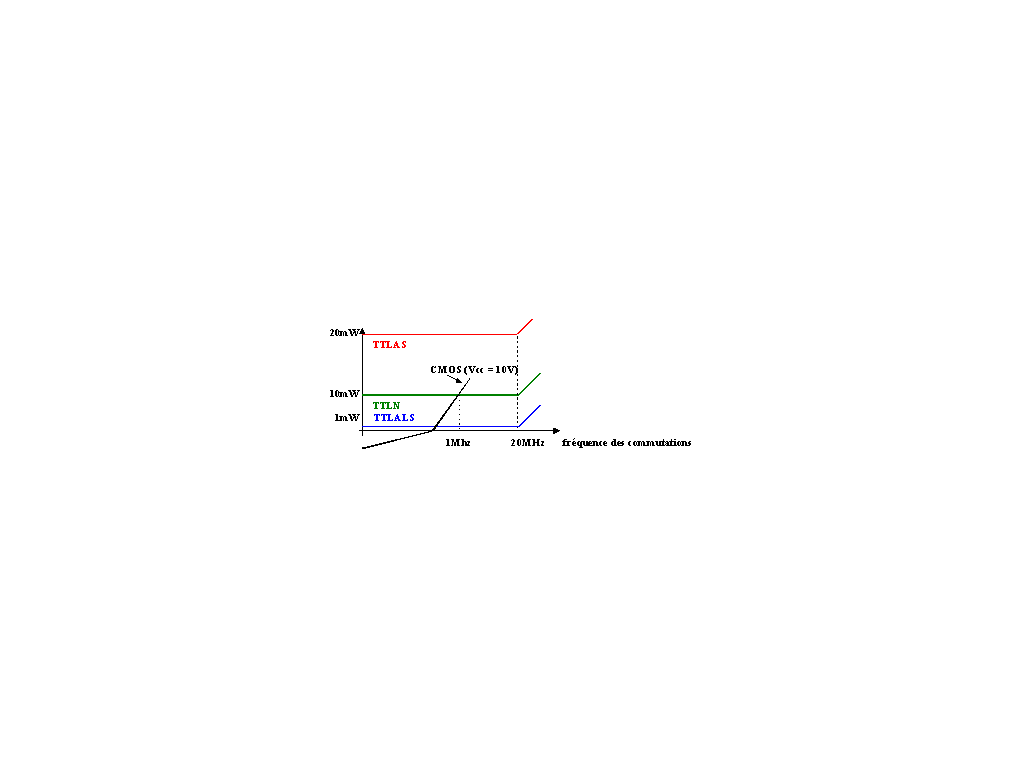
\includegraphics[width=\textwidth]{./images/cmos_tp.png}
      \caption{TP vs Vcc}
    \end{figure}
\end{frame}



\begin{frame}
  \frametitle{Digital Electronics Basics}
  \framesubtitle{Considering a real problem}
  \begin{block}{Implementation using Electronic component}
    \begin{itemize}
	\item Which Family? CMOS or TTL technology?
	\item Find components you need and correspoding datasheet
    \end{itemize}
  \end{block}

    \begin{figure}
      \centering
      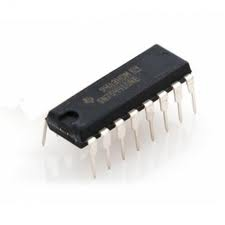
\includegraphics[width=.2\textwidth]{./images/ttl_7406.png}
      \caption{TTL 7406}
    \end{figure}
\end{frame}

\begin{frame}
  \frametitle{Digital Electronics Basics}
  \framesubtitle{Considering a real problem}
  \begin{block}{Implementation using Electronic component}
    \begin{itemize}
	\item Which Family? CMOS or TTL technology?
	\item Find components you need and correspoding datasheet
	\item Make the wiring of the circuit
    \end{itemize}
  \end{block}

    \begin{figure}
      \centering
      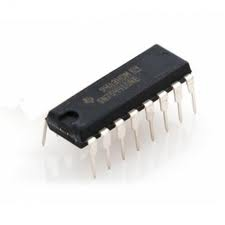
\includegraphics[width=.2\textwidth]{./images/ttl_7406.png}
      \caption{TTL 7406}
    \end{figure}
\end{frame}

%\subsection{Second subsection}
%
%\begin{frame}
%  \frametitle{A Kick-Ass Title}
%  \framesubtitle{A Kick-Ass Title Subtitle}
%  \begin{block}{Block environment}
%    \begin{itemize}
%    \item[\cross] Cross item
%    \item[\tick] Tick item
%    \end{itemize}
%  \end{block}
%  \begin{equation}
%    \label{eq:eq1}
%    f(x)=ax+b \ .
%  \end{equation}
%\end{frame}


\end{document}
